\documentclass{beamer}

\usepackage{multicol}

% to get a visual visula clue on how many slides are left
\usetheme[progressbar=frametitle]{metropolis}
% add the progressbar as fraction (E.g 1/3)  
\setbeamertemplate{frame numbering}[fraction]
\useoutertheme{metropolis}
\useinnertheme{metropolis}
\usefonttheme{metropolis}
\usecolortheme{spruce}
\setbeamercolor{background canvas}{bg = white}

\title[- short title -]{Your Title Here}
\subtitle{Subtitle Here}
\author{Your Name}
\institute{Institute Name}
\date{}    % No date but you can put a date or \today

% set transparency of the items displayed in conjunction with onslide
\setbeamercovered{transparent=15}

\begin{document}
% visually set blocks inside a frame in a colorbox
\metroset{block = fill}

\begin{frame} % in beamer you a frame can contain one or more slides

\titlepage

\end{frame}

\begin{frame}[t]{Functions} \vspace{4pt}

\begin{block}{Definition of a function}

\vspace{4pt}

A function is a function that is different from all functions

\vspace{4pt}

\end{block}


\end{frame}

\begin{frame}

% Set $D$ is called the \line(1, 0){50} of the function

% the above question is implemented as line in first slide
% and question with proper answer(domain) on the next slide

Set $D$ is called the
\only<1>{\line(1, 0){50}}
\only<2>{\textcolor{magenta}{domain}}
of the function

\end{frame}

\begin{frame}{Yet another title} \vspace{10pt}

% below line will take care of the alignment acc. text width
\begin{columns}[onlytextwidth]

% first column start
\column{0.4\textwidth}

$\sqrt{x^2} = $ \\[10pt]

\begin{enumerate}[(A)]	% A, B, C instead of numbers

\item $x$
\item $-x$
\item $|x|$

\end{enumerate}

% first column end

% second column start
\column{0.6\textwidth}

% include a case equation which appears only in slide 3
\only<3>
{
$
\sqrt{x^2} = 
\begin{cases}
-x, & x<0 \\ % & is used to align eqn right of comma
x, & x\geq 0 % & is used to align eqn right of comma
\end{cases}
$ 
\\[10pt]
}

% add image which appears after 2(including 2) for the current frame
\only<2->
{
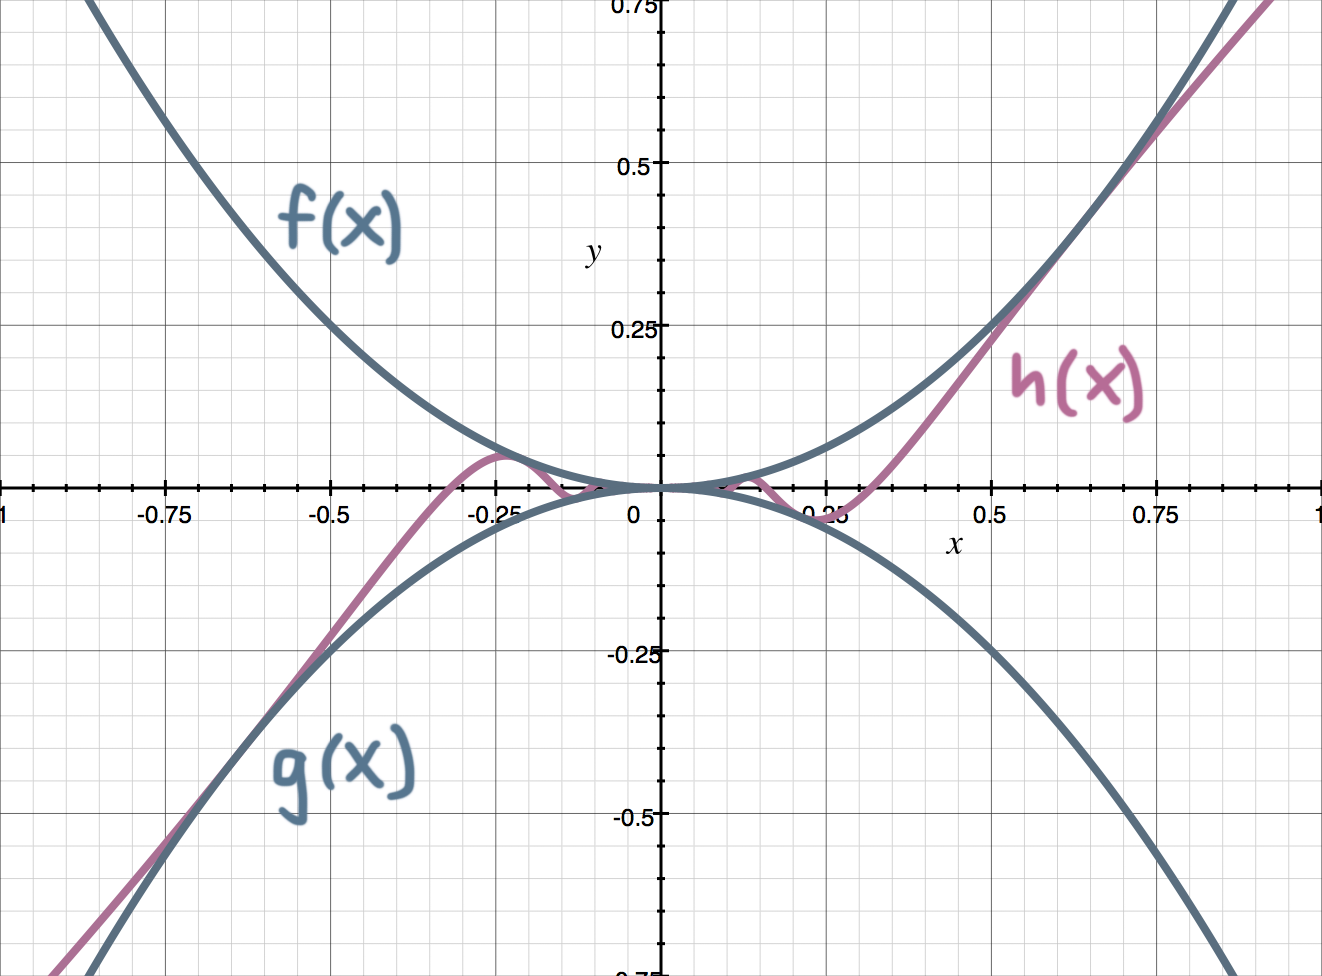
\includegraphics[width=0.6\textwidth]{limit}
}
% second column end

\end{columns}

\end{frame}

\begin{frame}[t]{Parent Functions} \vspace{4pt}

Name and sketch graph for each of the functions:

\begin{enumerate}

% multicols work best with enumeration multicol package required

\begin{multicols}{3}

% lets display all 15 items 5 at a time in a slide
% can also set transparency of the items which are displayed
% using \setbeamercovered{transparent=15} in preamble
% better than \only because content is only hidden hence
% it doesn't mess with styling while displaying item one by one

\item $y = x $
\item $y = |x| $
\item $y = x^2 $
\item $y = x^3 $
\item $y = x^b $

% display this from slide 2 onwards
\onslide<2->
{
\item $y = \sqrt{x} $
\item $y = \sqrt[3]{x} $
\item $y = \frac{1}{x} $
\item $y = 2^x $
\item $y = e^x $
}


% display this from slide 3 onwards
\onslide<3->
{
\item $y = \ln x $
\item $y = \frac{1}{1+e^{-x}} $
\item $y = \sin x $
\item $y = \cos x $
\item $y = \tan x $
}

\end{multicols}

\end{enumerate}

\end{frame}

\begin{frame}[standout]

\flushleft
Homework: p.342 \#7-21

\end{frame}

\end{document}